\section{Ziel}
Das Ziel dieses Versuchs ist es, aus einer Metalloberfläche
(Wolfram) durch Erwärmung freie Elektronen zu erzeugen und
daraus die Temperaturabhängigkeit dieses Vorgangs sowie die
Austrittsarbeit für Wolfram zu bestimmen.

\noindent Es soll außerdem die Hochvakuumdiode behandelt werden,
indem die Kennlinien dieser Diode untersucht werden.

\section{Theorie}
\label{sec:Theorie}

\subsection{Austrittsarbeit und die Energieverteilung der Leitungselektronen}

Atome sind in Metallen auf ihren Kristallgitterplätzen 
ionisiert. Es gibt dabei freie Elektronen außerhalb 
der periodischen Gitter. Diese werden als Leitungselektronen 
bezeichnet. Das Gitterpotential kann in grober Näherung als 
konstant betrachtet werden. Das Metallinnere hat ein positives 
Potential, das vom Außenbereich um einen Betrag $\phi$ 
verschieden ist. Man kann dies wie in Abb. \ref{fig:topf}
als Potentialtopf darstellen. Wenn ein Elektron diesen Topf 
verlassen möchte, muss es gegen das Potential $\zeta$ 
anlaufen können. Es muss also die Austrittsarbeit $e_0 \zeta$ %wirklich zeta?
aufbringen können. 

\begin{figure}
    \centering
    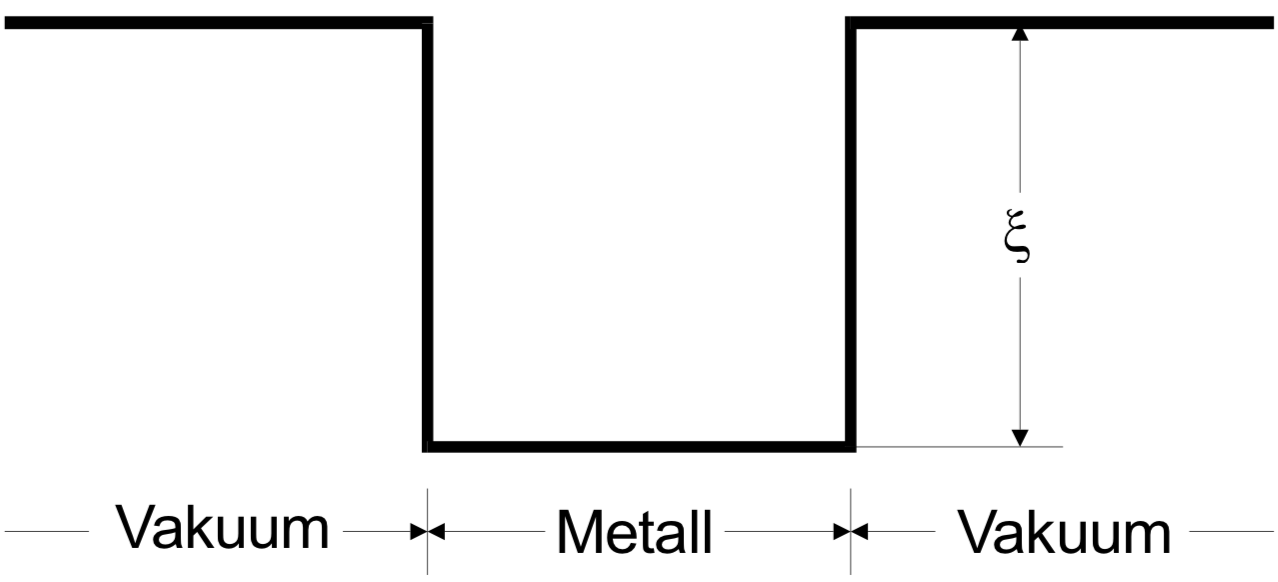
\includegraphics[width=6cm, height=3cm]{build/potentialtopf.png}
    \caption{Potentialtopf-Modell eines Metalls. \cite{V504}}
    \label{fig:topf}
\end{figure}

\noindent Aus der Quantentheorie ergibt sich, dass bei Zimmertemperatur 
die Fermische Grenzenergie $\zeta$ für alle Metalle größer ist 
als $k T$. Wie in Abb. \ref{fig:fermidirac} zu erkennen, muss
ein Elektron mindestens die Energie $\zeta + e_0 \Phi$ 
erbringen, um sich von der Metalloberfläche zu lösen. 

\noindent Als Näherung gilt 
\begin{equation}
    f(E) = exp{\frac{\zeta - E}{k T}}
    \label{eqn:fermidirac}
\end{equation}
für die Wahrscheinlichkeitsverteilung, dass ein Elektron die 
Oberfläche  verlässt. 

\begin{figure}
    \centering
    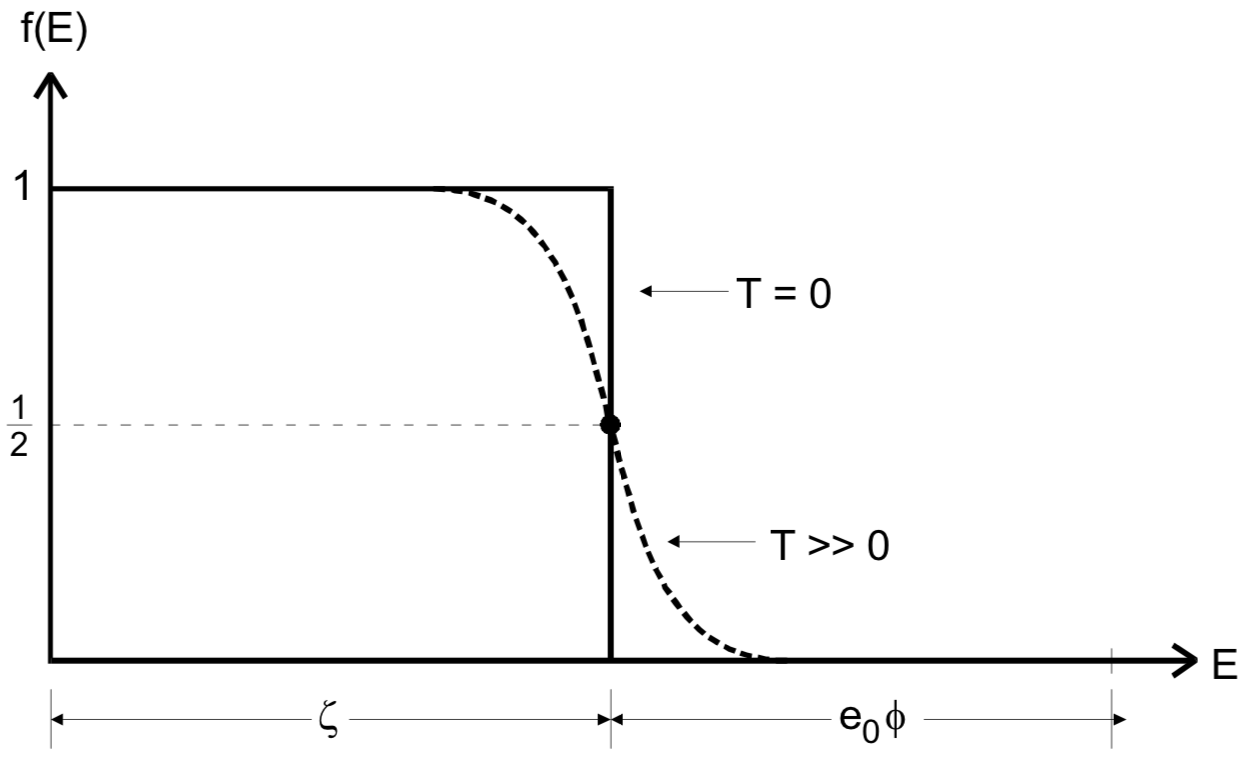
\includegraphics[width=10cm, height=6cm]{build/fermidirac.png}
    \caption{Verlauf der Fermi-Diracschen Verteilungsfunktion. \cite{V504}}
    \label{fig:fermidirac}
\end{figure}

\subsection{Berechnung der Sättigungsstromdichte bei der 
thermischen Elektronenemission}

Die Sättigungsstromdichte ist die Zahl der 
Elektronen, die pro Zeit- und Flächeneinheit aus der 
Metalloberfläche austreten. Diese ist abhängig von der 
Temperatur. Mittels einiger Umformungen und 
Zusammenhänge aus der Quantenmechanik ergibt sich die 
Richardson-Gleichung für die gesuchte Stromdichte $j_\text{S}(T)$:
\begin{equation}
    j_\text{S}(T)= 4 \pi \frac{e_0 \, m_0 \, k^2}{h^3} \, T^2 \, exp{\frac{-e_0 \, \Phi}{k \, T}}.
    \label{eqn:richardson}
\end{equation} 
Dabei ist $e_0$ die Ladung des Elektrons und $m_0$ seine Masse. 
Das Planksche Wirkungsquantum wird mit $h$ abgekürzt, $k$ ist 
die Boltzmann-Konstante und $\Phi$ ein Potential. %Keine Ahnung ob das so ist haha

\subsection{Hochvakuum-Diode}

Die Messung des Sättigungsstroms einer emittierenden 
Metalloberfläche muss im Hochakuum durchgeführt werden, 
damit die freien Elektronen nicht mit Luftmolekülen in 
Wechselwirkungen treten. Der grundsätzliche Aufbau einer 
Hochvakuum-Diode ist in Abb. \ref{fig:diode} zu erkennen.
Es wird eine Heizspannung an die Kathode angelegt. Dadurch 
lösen sich Elektronen und bewegen sich in Richtung der Anode. 
An der Anode ist eine Saugspannung angeschlossen, um das 
Gegenfeld zu verringern. Ist dieses zu groß, kommen die 
Elektronen nicht bei der Anode an. 

\begin{figure}
    \centering
    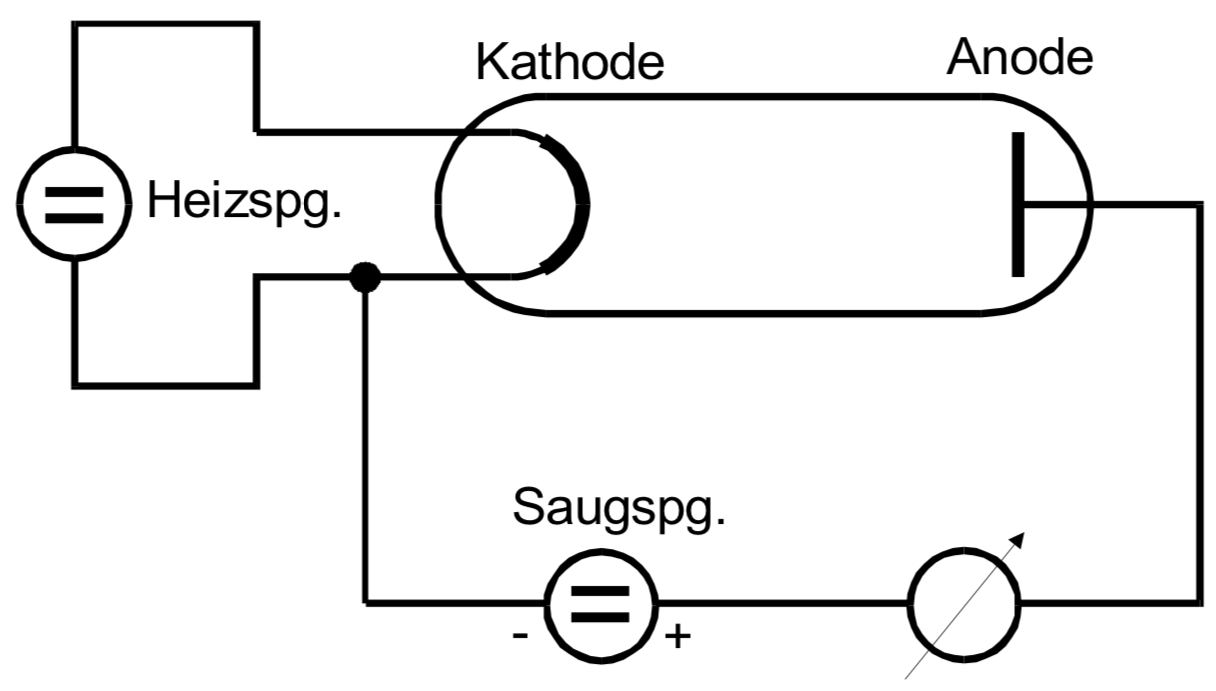
\includegraphics[width=8cm, height=4cm]{build/diode.png}
    \caption{Schaltung einer Hochvakuumdiode. \cite{V504}}
    \label{fig:diode}
\end{figure}

\subsection{Die Langmuir-Schottkysche Raumladungsgleichung}

Der Anodenstrom hängt neben 
der Kathodentemperatur auch noch von der Anodenspannung 
ab. Außerdem ist die Geschwindigkeit der Elektronen nicht 
konstant. Es handelt sich stattdessen um eine beschleunigte 
Bewegung. Auch die Raumladungsdichte $\rho$ ist eine Funktion 
des Ortes und nimmt zur Anode hin ab. Dies gilt, da die 
Geschwindigkeit zunimmt und die Stromdichte $j$ konstant ist. 
Nach einigen Umformungen und einer Integration lässt sich aus 
der Potentialgleichung herleiten, dass sich der Zusammenhang 
zwischen der Stromdichte $j$ und der Anodenspannung $V$ 
zu 
\begin{equation}
    j = \frac{4}{9} \epsilon_0 \sqrt{2 \frac{e_0}{m_0}} \frac{V^{\frac{3}{2}}}{a^2}
    \label{eqn:langmuirschottky}
\end{equation}
ergibt. Diese Gleichung wird auch Langmuir-Schottkysches 
Raumladungsgesetz genannt. Der Gültigkeitsbereich ist das 
Raumladungsgebiet - wie in Abb. \ref{fig:langmuirschottky}
dargestellt.  

\begin{figure}
    \centering
    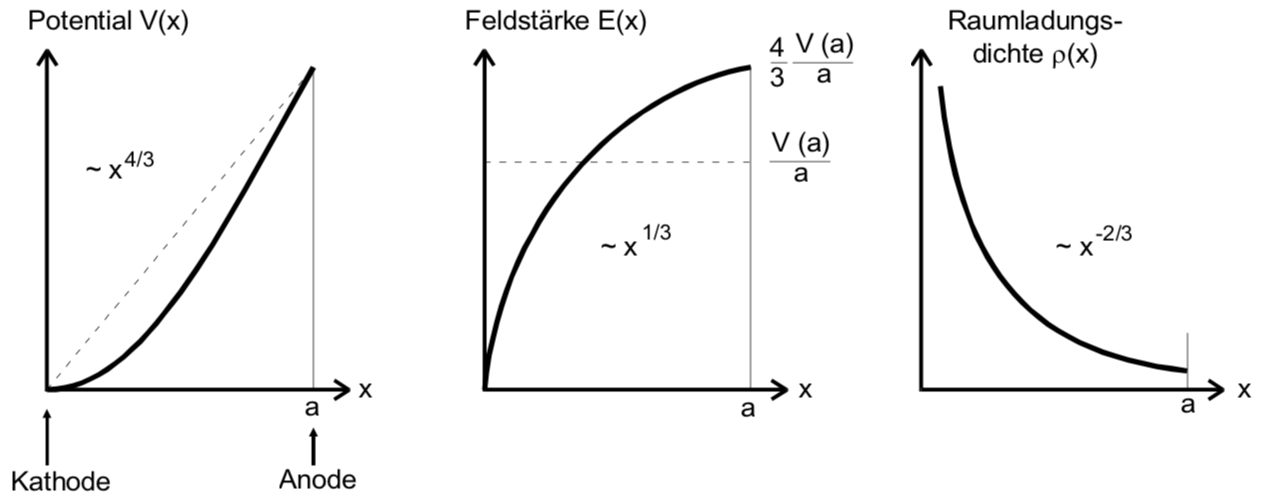
\includegraphics[width=13cm, height=5cm]{build/raumladungsgebiet.png}
    \caption{Potential, Feldstärke und Raumladungsdichte im Raumladungsgebiet
        einer Hochvakuumdiode. \cite{V504}}
    \label{fig:langmuirschottky}
\end{figure}

\subsection{Anlaufstromgebiet einer Hochvakuumdiode}

Es wird bei $V = 0$ noch ein geriner Anodenstrom gemessen, 
obwohl zu erwarten wäre, dass $j = 0$ gilt. Dieser entsteht 
durch die Eigengeschwindigkeit der Elektronen. Bei $T > 0$ 
gibt es viele Elektronen, deren Energie größer als die 
Austrittsarbeit ist. Diese Differenz wird als kinetische 
Energie umgesetzt. Damit sind sie in der Lage gegen ein 
geringes Gegenfeld zu laufen - daher der Name Anlaufstrom. 
Die Energieverhältnisse sind in Abb. \ref{abb:energie}
dargestellt. Dabei ist wichtig, dass das Anodenmaterial auch 
eine Austrittsarbeit besitzt. Durch die leitende Verbindung 
zwischen Anode und Kathode werden die Fermi-Oberflächen auf 
eine Höhe gebracht.Durch das äußere Potential $V$ 
verschieben sie sich um $e_0 V$.

\begin{figure}
    \centering
    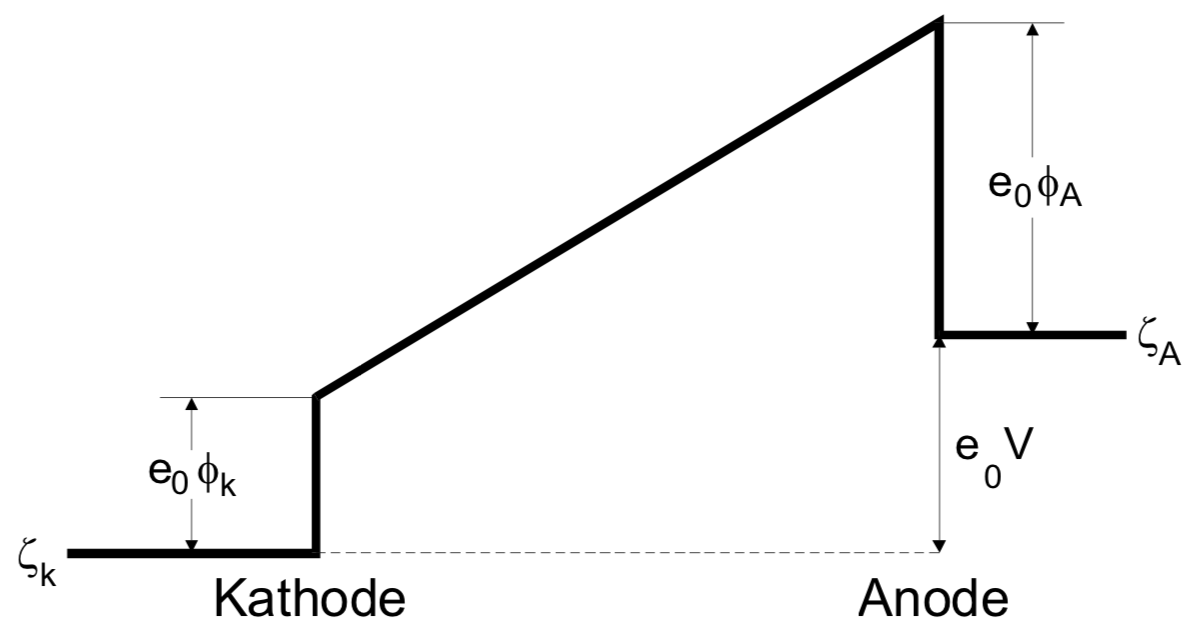
\includegraphics[width=10cm, height=6cm]{build/energie.png}
    \caption{Energieverhältnisse in der Hochvakuumdiode im Anlaufstromgebiet. \cite{V504}}
    \label{fig:energie}
\end{figure}

\noindent Die Abhängigkeit der Anlaufstromstärke vom äußeren
Potential ist durch folgende Gleichung darstellbar
\begin{equation}
    j(V) = const \, exp{-\frac{e_0 \, V}{k \, T}}.
    \label{eqn:anlauf}
\end{equation}

\subsection{Kennlinie der Hochvakuumdiode}

Die Kennlinie wird als der Zusammenhang zwischen Anodenstrom 
$I_\text{A}$ und dem angelegten Potential bezeichnet. 
Sie lässt sich in Anlaufstrom-, Raumladungs- und 
Sättigungsstromgebiet gliedern. 
Diese Abschnitte sind in Abb. \ref{fig:gebiete} zu erkennen.
Aus der Kennlinie lassen sich Kathodentemperatur und die 
Austrittsarbeit der Kathode ermitteln.

\begin{figure}
    \centering
    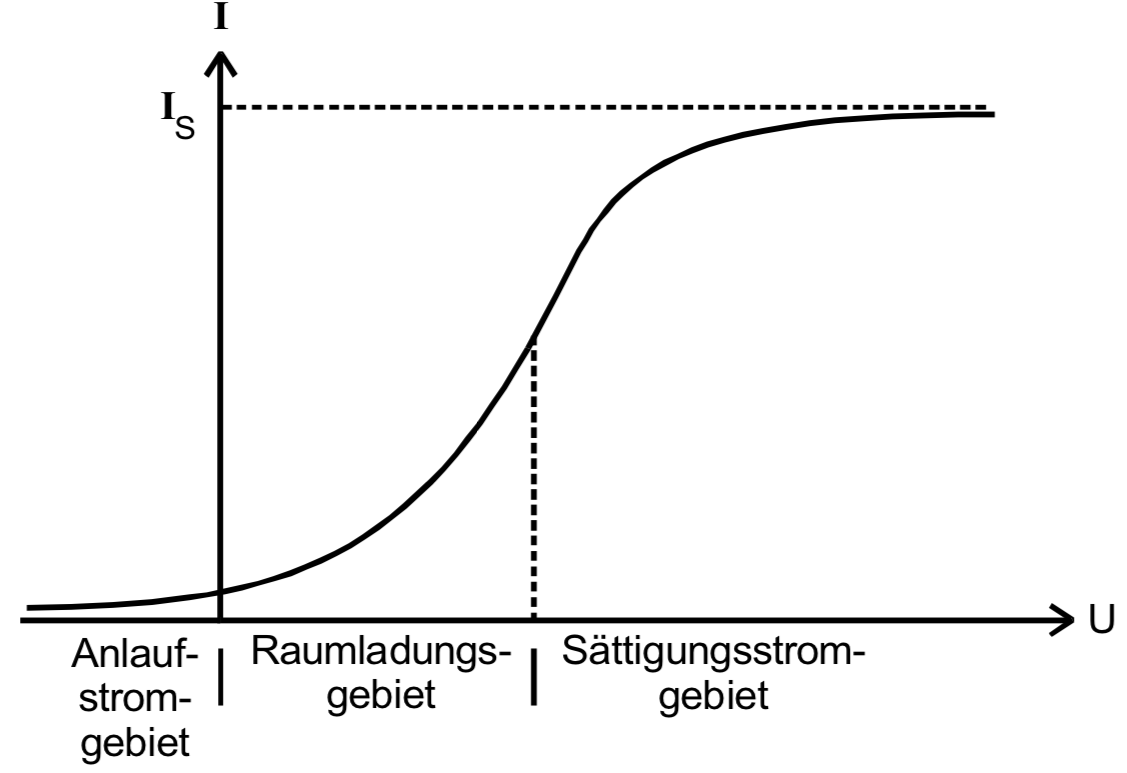
\includegraphics[width=10cm, height=7cm]{build/gebiete.png}
    \caption{Kennlinie einer Hochvakuumdiode. \cite{V504}}
    \label{fig:gebiete}
\end{figure}


\subsection{Temperaturberechnung} %umbenennen?
Das Stefan-Boltzmannsche Gesetz lautet
\begin{equation*}
    N = f \, \eta \, \sigma \, T^4.
\end{equation*}
Dabei ist $\sigma$ die Stefan-Boltzmannsche Strahlungskonstante,
welche einen Wert von
\begin{equation*}
    \sigma = \SI{5.7e-12}{\watt\per\centi\meter\squared\per\kelvin\tothe{4}}
\end{equation*}
hat, $f$ die emittierende Kathodenoberfläche, $\eta$ der
Emissionsgrad der Oberfläche und $T$ die Temperatur.

\noindent Aus dem Energiesatz folgt
\begin{equation*}
    I_\text{H} \, U_\text{H} = f \, \eta \, \sigma \, T^4 \, + \, N_\text{WL}.
\end{equation*}
Dabei ist $N_\text{WL}$ die Wärmeleitung, für die ein Wert von
$N_\text{WL} = \SI{1}{\watt}$ angenommen wird.
Also lässt sich daraus die Temperatur durch
\begin{equation}
    T = \sqrt[4]{\frac{I_\text{H} \, U_\text{H} - 1}{f \, \eta \, \sigma}}
    \label{eqn:Temp}
\end{equation}
berechnen.

%Lineare Regression erklären?